\chapter{Angle Measurement with Built-in Sensors}\label{chap:CompFilter}
It is a goal to get the Cubli setup to balance the frame in an upright position independently of the baseplate orientation feasible limits.

As described in \secref{sec:Sensors} there are two IMUs mounted on the frame of the Cubli (shown on \figref{CubliParts}). They can be used to achieve this goal since they only depend on the absolute angle and they can also be used in the full Cubli. In this case it has been decided to use IMU number one for the calculations, but number two would be valid too.

\section{Angle Calculations from the IMUs}
The angular position of the Cubli can be calculated using the accelerometer, the gyroscope or combining both. In this section each of the options is described and analyzed.

\subsection{Angle from the Accelerometer}
The accelerometer measures linear acceleration, and if the accelerometer is attached to a object that does not accelerate with respect to the Earth, the accelerometer will measure the gravitational acceleration. This can be used to determine the orientation of the accelerometer sensor with respect to the Earth \cite{JWarren}.\\
The accelerometers used with the Cubli setup have 3-axis detection as described in \secref{sec:Sensors}. To determine the angle of the frame (\si{accel\_\theta_{F}}) with the accelerometer it is needed to get the measurements from two of the three axes. The two measurements needed are the ones in line with the frames movement direction, based on the way the IMU is mounted, as shown in \figref{accelerometer}. 

\begin{minipage}{\linewidth}
	\begin{minipage}{0.45\linewidth}
		\begin{figure}[H]
			\centering
			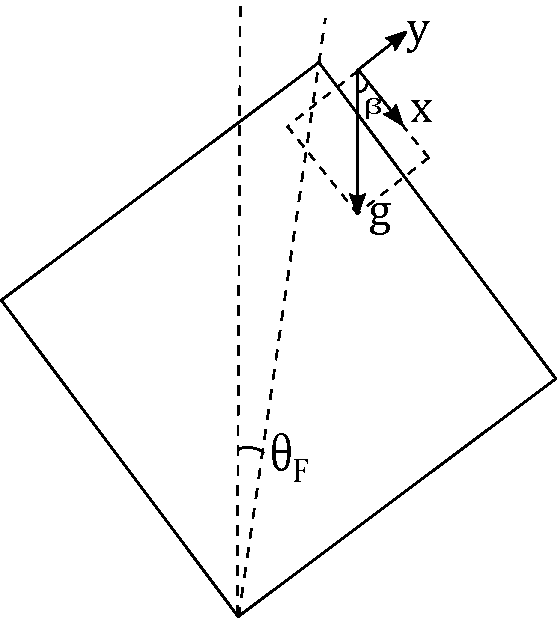
\includegraphics[scale=0.58]{figures/accelerometer}
			\captionsetup[subfigure]{font = footnotesize}
			\captionof{figure}{Position of the IMU on the setup. The orientation of the accelerometer in relation to the Cubli frame is shown. The sensor is rotated by \si{\frac{\pi}{4}} in relation to the angle \si{\theta_F}. On the IMU the components of the acceleration vector are shown. In case of no movement of the frame these are the components of the gravitational acceleration vector.}
			\label{accelerometer}
		\end{figure}\vspace{-5mm}
	\end{minipage}
	\hspace{0.03\linewidth}
	\begin{minipage}{0.45\linewidth}
		\begin{figure}[H]
			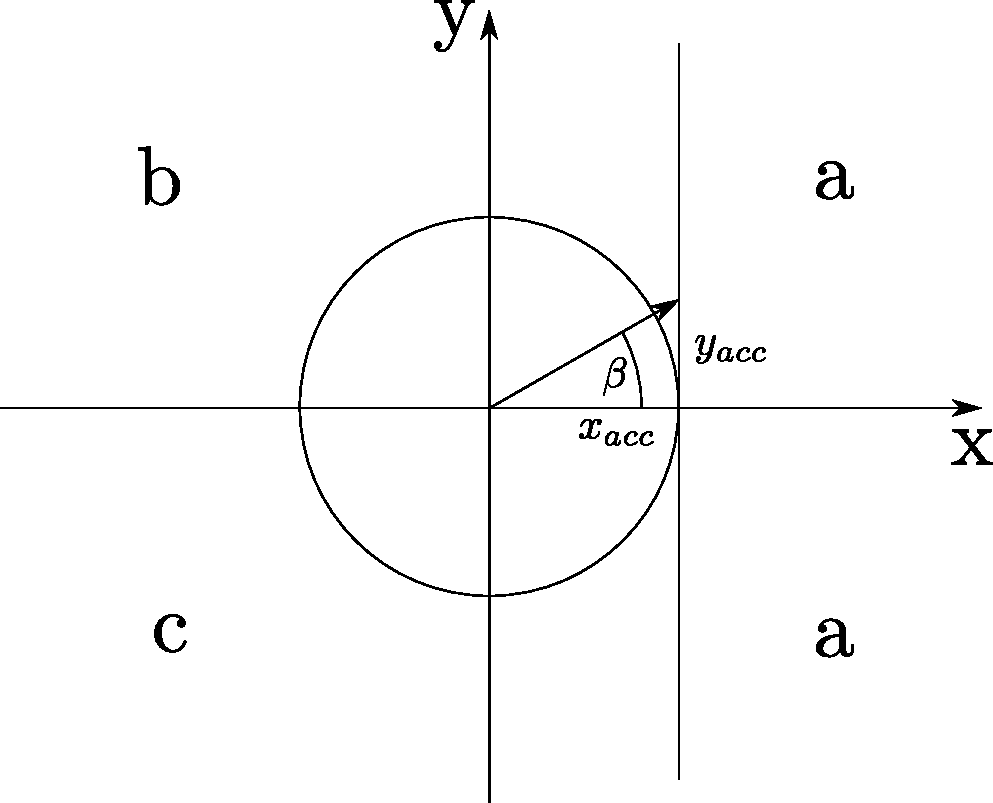
\includegraphics[scale=.425]{figures/tangentCircle}
			\centering
			\captionsetup[subfigure]{font = footnotesize}
			\captionof{figure}{atan() is only valid as long as x is positive (a), where the angle (\si{\beta}) is found through the inverse tangent \si{\beta = \arctan\left(\frac{y}{x}\right)} . If the frame moves more than \si{45^\circ} from equilibrium, then the IMU will have x or y move outside the two areas indicated with a. Angle calculation for area b is \si{\beta = \pi - \arctan\left(\frac{y}{x}\right)} and for c it is \si{\beta = \arctan\left(\frac{y}{x}\right) - \pi}. } 
			\label{accelImplementation}
		\end{figure}
	\end{minipage}
\end{minipage}

Based on the markings on the IMU, those are the x- and y-axis components of the linear acceleration. Taking the two axis measurements shown in \figref{accelerometer} and the different calculations of \si{\beta} depending on x and y (see \figref{accelImplementation}), the angle can be found using \eqref{accelAngle} \cite{CFisher}. 
%
\begin{flalign}
	\eq{accel\_\theta_{F}} {\beta + \frac{\pi}{4}} \unit{rad} 
	\label{accelAngle}
\end{flalign}
%
\hspace{6mm} Where:\\
\begin{tabular}{ p{1cm} l l l}
	& \si{\beta}& is the angle between the x component and the gravity vector		& \unitWh{rad}	\\
%	& x			& is the x component of the measured linear acceleration   & \unitWh{m \cdot s^{-2}} \\  
%	& y			& is the y component of the measured linear acceleration   & \unitWh{m \cdot s^{-2}} \\                   
\end{tabular} \\
\\
The offset (\si{\frac{\pi}{4}}) is added because the IMU is mounted with a \si{\frac{\pi}{4}} rotation compared to the orientation of the frame.

A test to measure the angle of the frame with the accelerometer is performed, with the purpose of comparing it to data from the potentiometer. The data from both sensors is read at the same time, to make it possible to compare the accelerometer to the potentiometer to determine if the accelerometer can be used instead of the potentiometer.\\
A comparison of the two measurements is shown in \figref{angleAcc}. The accelerometer angle (\si{accel\_\theta_{F}}) is found by taking the x- and y-axis components and calculating the angle with \eqref{accelAngle}.
The data of the test can be found in  \appref{app:IMUMeasurementsAppendix}. 
%
\begin{figure}[H]
	\centering
	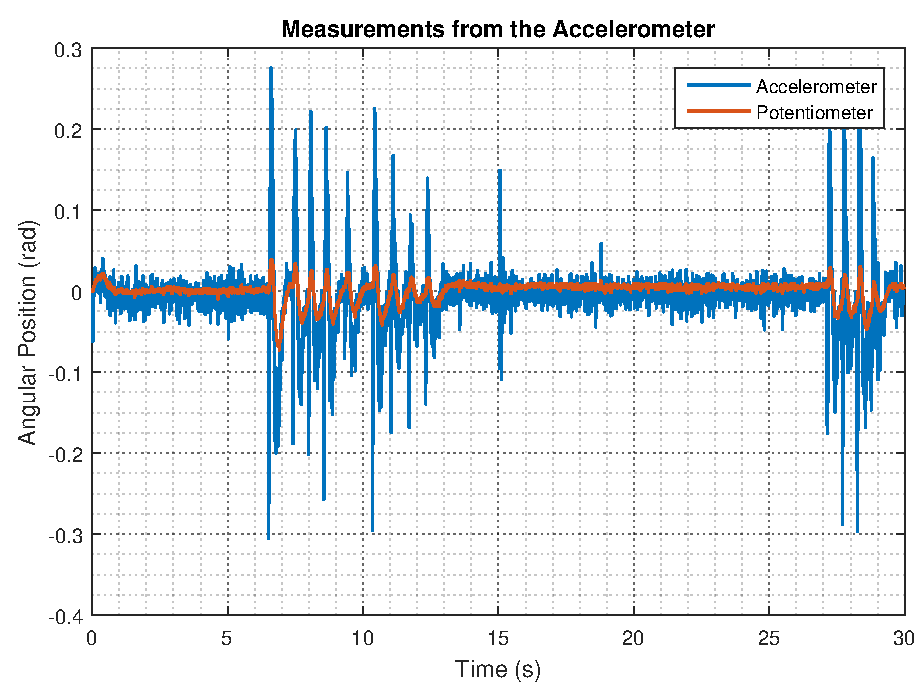
\includegraphics[scale=0.65]{figures/angleAcc}
	\caption{The graph shows a comparison of the angle of the frame measured by the potentiometer (orange) and the same angle found with the accelerometer (blue). The accelerometer angle is calculated based on the data from the x- and y-axis components (\appref{app:IMUMeasurementsAppendix})}
	\label{angleAcc}
\end{figure}\vspace{-5mm}
%
The measurements of the potentiometer and accelerometer are both showing the Cubli frame in the same position. It can be seen that the calculations from the accelerometer has a lot more noise than the potentiometer.

While the Cubli setup tries to balance the frame, the IMU mounted on the top of it will move along with the frame. The spikes are present on the calculated angle from the accelerometer data in \figref{angleAcc} due to the acceleration of the frame that creates a disturbance on the measurement of the gravitational acceleration \cite{JWarren}.\\
A way to minimize this disturbance would be to move the IMU as close as possible to the point of rotation. This way the accelerometer is still able to measure the gravitational acceleration, but the distance to the pivoting point is  shorter and the linear acceleration will be smaller. However, since the design should be portable to the full Cubli, where the pivoting point is always changing, this solution does not seem to be adequate.

\subsection{Angle from the Gyroscope}
The angle of the frame could also be found with the gyroscope (\si{gyro\_\theta_{F}}), by integrating the measured angular velocity on the axis aligned with the direction of motion of the frame as shown in \figref{cubliMechanical}.

\begin{flalign}
	\eq{gyro\_\theta_{F}[n]} {\int_{0}^{n\cdot \Delta T} \omega_{F} \, \mathrm{d}t}
	\label{accelGyro}
\end{flalign}
\hspace{6mm} Where:\\
\begin{tabular}{ p{1cm} l l l}
	& \si{\omega_{F}}			& is the measured angular velocity of the frame  & \unitWh{rad \cdot s^{-1}} \\  \\                       
\end{tabular} 
\\
The problem with the data from the gyro is an accumulating error which is caused by the integration done to convert angular velocity into an usable angle. It is also known that the gyros will exhibit a drifting error when experiencing small and slow movement \cite{JWarren}. These problems can be observed in \figref{angleGyro}.
\begin{figure}[H]
	\centering
	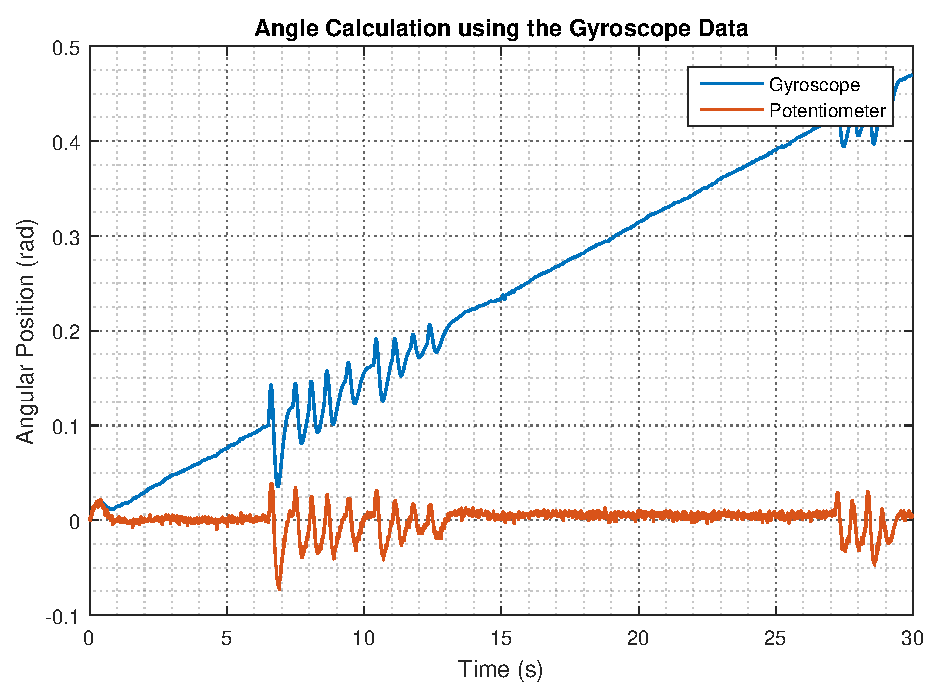
\includegraphics[scale=0.65]{figures/angleGyro}
	\caption{Angular position calculation with the data of the gyroscope}
	\label{angleGyro}
\end{figure}\vspace{-5mm}
%The problem with the data from the gyro is it will exhibit a drifting error when experiencing no movement \cite{JWarren} and since the angular velocity has to be integrated to get the angel there will be an accumulation error. 

Assuming that the drift is proportional to time (the slope is always constant), a way to minimize its influence on the data would be to do a test while keeping the frame motionless. The inclination of the slope from the data graph multiplied with the sampling time is then the offset that has to be subtracted from each measurement.

It can also be calculated online, while the controller is running. In this case the accelerometer can provide information to compensate this drift. One solution to fuse these two sets of data is to use a complementary filter, explained in detailed in next section.

\subsection{Data Fusing with Complementary Filter}
In order to filter the drift of the gyroscope and the disturbance errors of the accelerometer, a complementary filter can be used to combine both measurements. This is done to get a more reliable angle measurement for both when the frame is moving and when its standing still in the equilibrium point.\\
The two angle measurements of the IMU are sent through a filter and then summed in order to get an angle of the Cubli's frame. This will result in relying more in the accelerometer data when there is a slow movement and more in the gyroscope when the movement is fast.\cite{PGui}

\begin{figure}[H]
	\begin{tikzpicture}[ auto,
thick,                         %<--setting line style
node distance=2cm,             %<--setting default node distance
scale=1.5,                     %<--|these two scale the whole thing
every node/.style={scale=1.5}, %<  |(always change both)
>=triangle 45 ]                %<--sets the arrowtype
\draw%--------------------------------------------------------------------------------------------

node[shape=coordinate][](acc) at (0,0){acc}			% start of acc signal path

node(lowpas) at (6,0) [block] {\Large $\ \frac{1}{\tau \cdot s + 1}$ }

node[shape=coordinate][](gyro) at (0,-2){}		% start of gyro signal path

node(integrate) at (3,-2) [block] {\Large $\frac{1}{s}$}

node(highpas) at (6,-2) [block] {\Large $\ \frac{\tau \cdot s}{\tau \cdot s + 1}$ }

node(sum) at (8,-1) [sum] {$\sum$}


node[shape=coordinate][](angle) at (10,-1){}		% output of the complementary filter
;

\draw[->](acc) -- node {accel$\_\theta_{F}$} (lowpas);
\draw[->](gyro) -- node {gyro$\_\omega_{F}$} (integrate);
\draw[->](integrate) -- node {} (highpas);

\draw[->](highpas) -| node {} (sum);
\draw[->](lowpas) -| node {} (sum);


\draw[->](sum) -- node {$\theta_{F}$} (angle);

\end{tikzpicture}

	\centering
	\caption{Block diagram of the complementary filter setup used for the IMU on the Cubli. The calculated accelerometer angle passes through a low pas filter. The angular velocity measurement from the gyro is integrated and then passed through a high pass filter. Both measurements are then summed to get the angle of the frame. \si{tau} refers to the time constant of the filters.}
	\label{blockDrawingComplementaryFilter}
\end{figure}
%
The filter for the IMU is designed as shown in \figref{blockDrawingComplementaryFilter} with a low pass filter on the measurements from the accelerometer, and an integration followed by a high pass filter on the measurements from the gyroscope \cite{OlliW}.\cite{PGui}
\begin{flalign}
	\eq{\theta_{F}} {\frac{1}{ 1 + \tau \cdot s} \cdot accel\_\theta_{F}}   &\\
	\eq{\theta_{F}} {\frac{\tau \cdot s}{ 1 + \tau \cdot s} \cdot \frac{1}{s} \cdot gyro\_\dot{\theta}_{F}}	&
	\label{complementaryBlockFilters}
\end{flalign}
Combining the two equations yields \eqref{complementaryCombinedFilter}
\begin{flalign}
	\eq{\theta_{F}} {\frac{1}{ 1 + \tau \cdot s} \cdot accel\_\theta_{F} + \frac{\tau \cdot s}{ 1 + \tau \cdot s} \cdot \frac{1}{s} \cdot gyro\_\dot{\theta}_{F} = \frac{accel\_\theta_{F} + \tau \cdot gyro\_\dot{\theta}_{F}}{1 + \tau \cdot s}} &
	\label{complementaryCombinedFilter}
\end{flalign}
Where \si{\tau} is the time constant of the filters. %Changing this constant decides how much the two different sensor measurements weight in on the combined angle.
 
\section{Discretization of the Complementary Filter} 
In order to use the complementary filter on the Cubli it needs to be discretized. This is done with the bilinear transformation method, where \si{s = \frac{2}{\Delta T}\cdot \frac{1 - z^{-1}}{1 + z^{-1}}}, with a sample time of \SI{10}{ms}.
Rewriting \eqref{complementaryCombinedFilter} yields
\begin{flalign}
 	\eq{\theta_{F}} {\frac{1}{1 + \tau \cdot s} \cdot (accel\_\theta_{F} + \tau \cdot gyro\_\dot{\theta}_{F})} &
 	\label{discreteComplementaryFilter1}
\end{flalign}
If s is replaced by its discrete expression the equation can be written in z-domain.
\begin{flalign}
  	\eq{\theta_{F}} {\frac{1}{1 + \tau \cdot \frac{2}{\Delta T}\cdot \frac{1 - z^{-1}}{1 + z^{-1}}} \cdot (accel\_\theta_{F} + \tau \cdot gyro\_\dot{\theta}_{F})} &
  	\label{discreteComplementaryFilter2}
\end{flalign}
%
%\begin{flalign}
%  	\eq{\Updownarrow \theta_{F}} {\frac{\Delta T \cdot (1 + z^{-1})}{\Delta T \cdot (1 + z^{-1})+2\cdot (1 - z^{-1})\cdot \tau} \cdot (accel\_\theta_{F} + \tau \cdot gyro\_\dot{\theta}_{F})}
%  	\label{discreteComplementaryFilter3}
%\end{flalign}
  %
\begin{flalign}
   	\eq{\theta_{F}} {\frac{\Delta T + \Delta T \cdot z^{-1}}{(2\cdot \tau + \Delta T) - (2\tau - \Delta T)\cdot z^{-1}} \cdot (accel\_\theta_{F} + \tau \cdot gyro\_\dot{\theta}_{F})} &
\end{flalign}\label{discreteComplementaryFilter4}
%
%\begin{flalign}
%	\eq{\Updownarrow \theta_{F} \cdot ((2\cdot \tau + \Delta T) - (2\tau - \Delta T)\cdot z^{-1})} {\Delta T + \Delta T \cdot z^{-1} \cdot (accel\_\theta_{F} + \tau \cdot gyro\_\dot{\theta}_{F})} &
%\end{flalign}\label{discreteComplementaryFilter5}
%%
Then \eqref{discreteComplementaryFilter4} is transformed from z-domain to discrete time domain, resulting in the difference equation.
% OLD 9.9
%\begin{flalign}
%	\eqOne{\theta_{F}[n] \cdot (2\cdot \tau + \Delta T) - \theta_{F}[n-1] \cdot (2\tau - \Delta T)} {\Delta T \cdot (accel\_\theta_{F}[n] + accel\_\theta_{F}[n-1]} 
%	\eqTwo{ + \tau \cdot gyro\_\dot{\theta}_{F}[n] + \tau \cdot gyro\_\dot{\theta}_{F}[n+1])} 
%	\label{discreteComplementaryFilter6}
%\end{flalign}
%  
\begin{flalign}
	\eqOne{\theta_{F}[n]}{\frac{(2\cdot \tau + \Delta T)}{2\cdot \tau + \Delta } \cdot \theta_{F}[n-1] + \frac{\Delta T}{2\cdot \tau + \Delta T} \cdot accel\_\theta_{F}[n] + \frac{\Delta T}{2\cdot \tau + \Delta T} \cdot accel\_\theta_{F}[n-1]} 
	\eqTwo{ + \frac{\Delta T \cdot \tau}{2\cdot \tau + \Delta T} \cdot gyro\_\dot{\theta}_{F}[n] + \frac{\Delta T \cdot \tau}{2\cdot \tau + \Delta T} \cdot gyro\_\dot{\theta}_{F}[n-1]} 
	\label{discreteComplementaryFilter7}
\end{flalign}
%

\section{Calculation of the Cut-off Frequency}
Based on the setup of the complementary filter in \figref{blockDrawingComplementaryFilter}, the same cut-off frequency is chosen for both low and high pass filter, since it is desired to find the angle of the frame with a gain of 1 (see \figref{bodeFilters}). As it can be seen in \figref{bodeFilters2}, if both filters have different cut-off frequencies the gain is less than one at some frequencies, which could be a problem in the calculation of the angular position of the frame. 

\begin{minipage}{\linewidth}
	\begin{minipage}{0.45\linewidth}
		\begin{figure}[H]
			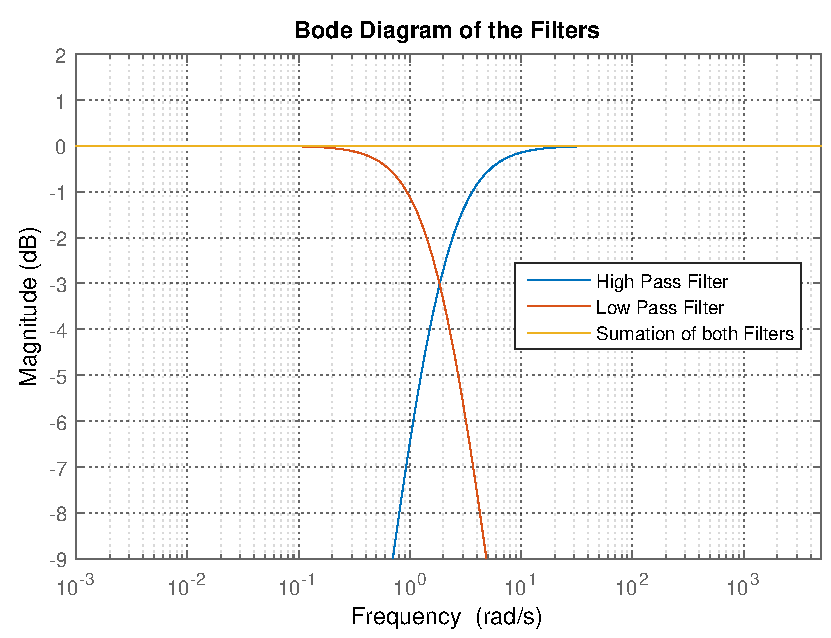
\includegraphics[scale=.55]{figures/bodeFilters}
			\centering
			\captionsetup{justification=centering}
			\captionof{figure}{Magnitude bode diagrams of the high pass and low pass filters with the same cut-off frequency as well as the summation of both}
			\label{bodeFilters}
		\end{figure}
	\end{minipage}
	\hspace{0.03\linewidth}
	\begin{minipage}{0.45\linewidth}
		\begin{figure}[H]\vspace{0mm}
			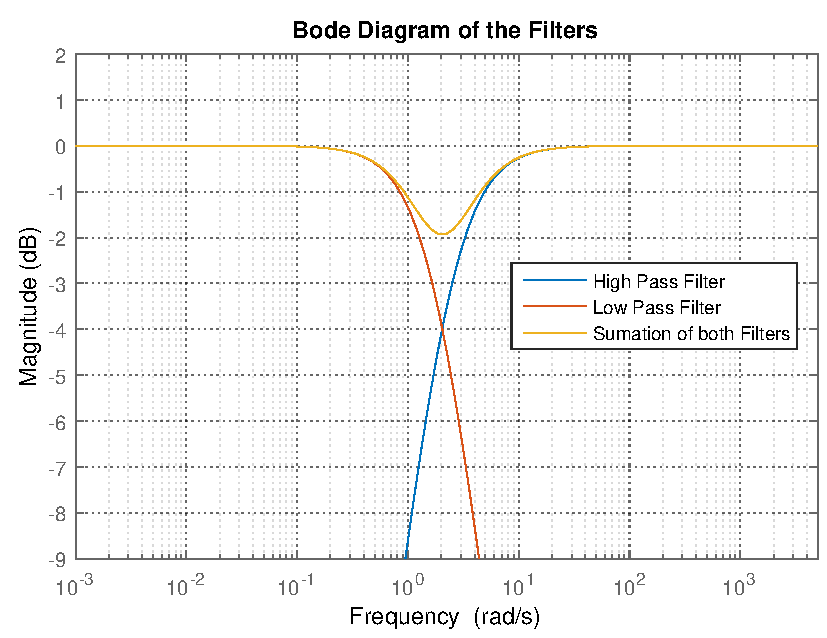
\includegraphics[scale=.55]{figures/bodeFilters2}
			\centering
			\captionsetup{justification=centering}
			\captionof{figure}{Magnitude bode diagrams of the high pass and low pass filters with different cut-off frequencies as well as the summation of both}
			\label{bodeFilters2}
		\end{figure}
	\end{minipage}
\end{minipage}

The cut-off frequency for the filters can be determined by using Senstools and the data obtained through the test detailed in \appref{app:IMUMeasurementsAppendix}.

The toolbox uses the data form the potentiometer as the real output of the system, the data from the IMUs as the input and the modeling of the system is done through \eqref{discreteComplementaryFilter7}. With this data Senstools can find the optimal value for \si{\tau} based on the difference between the angle measured by the potentiometer and an angle calculated from accelerometer and gyroscope measurements done during the same test.

The final fit can be seen in \figref{filterSensTool} and it gives an optimal \si{\tau=\ }\SI{0,5399}{s}. This results in a cut-off frequency for the filter equal to \si{1,85\ rad \cdot s^{-1}}.

%
\begin{figure}[H]
	\centering
	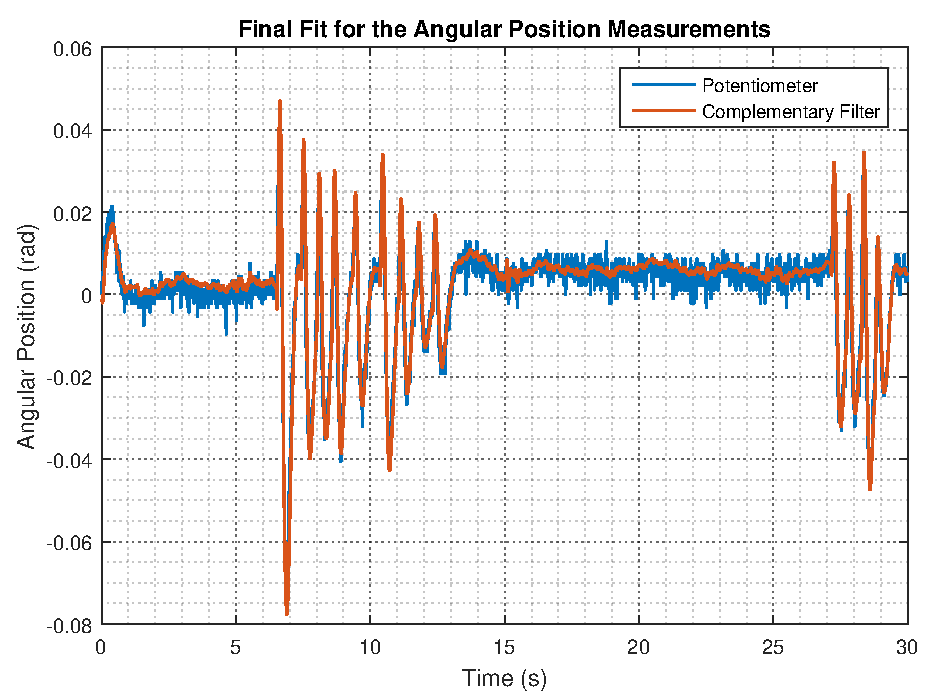
\includegraphics[scale=0.65]{figures/filterSensTool}
	\caption{Final result of the complementary filter compared with the data from the potentiometer. It can be observed that the two measurements match closely}
	\label{filterSensTool}
\end{figure}\vspace{-5mm}
%
%Using the same cut-off frequency for both filters has been successfully implemented and hence it there was not done any investigation into different cut-off frequencies for the low and high pass filter.\\

\section{Implementation of the Complementary Filter}
Implementing \eqref{discreteComplementaryFilter7} yields to following piece of code. 

\begin{lstlisting}[style = customcpp,
				caption  = {Code for the implementation of the complementary filter in C\texttt{++}},
				label    = codeCompFilter ]
//---------------------- IMU --------------------------//
double Imu::getPosition(double accAngleNow, double gyroVelocityNow, double Ts, int imuNb)
{
	const double acc_off_1 = 0.84;  	// accel meass offset
	const double tau = 0.5399;			// cut-off for the complementary filter

	// Coefficients for the complementary equation
	const double K1 = (2 * tau - Ts) / (2 * tau + Ts);
	const double K2 = Ts / (2 * tau + Ts);

	if(imuNb == 1) 
	{
		static double acc_angle_1[2] = {accAngleNow + acc_off_1, 0},
		gyro_angle_1[2] = {gyroVelocityNow, gyroVelocityNow},
		comp_angle_1[2] = {acc_angle_1[0], 0};

		// Set old measurement data
		acc_angle_1[1] = acc_angle_1[0];
		gyro_angle_1[1] = gyro_angle_1[0];
		gyro_angle_1[0] = gyroVelocityNow;
		comp_angle_1[1] = comp_angle_1[0];

		acc_angle_1[0] = accAngleNow + acc_off_1;

		//Complementary equation using Tustin
		comp_angle_1[0] = K1 * comp_angle_1[1] + K2 * (acc_angle_1[0] + acc_angle_1[1] + tau * gyro_angle_1[0] + tau * gyro_angle_1[1]);
		return comp_angle_1[0];
	}
}

\end{lstlisting}

The position is calculated through the function \lstinline[style=customcppinline]{getPosition()}. \\
First, the values for the offset of the accelerometer angle and the cut-off frequency are initialized, as well as the two constants for the filter, K1 and K2.\\
When this function is called the first time, accelerometer, gyroscope and angle arrays are initialized.\\
The old values from \lstinline[style=customcppinline]{accel_angle}, \lstinline[style=customcppinline]{gyro_angle} and \lstinline[style=customcppinline]{comp_angle} are moved up in their arrays and new data is saved in \lstinline[style=customcppinline]{gyro_angle} and \lstinline[style=customcppinline]{accel_angle} on index 0. \\
Finally, the equation of the complementary filter in implemented to get the angular position of the frame.
